\section{Resultados Obtidos}

Os resultados compreendem as etapas de avalização e implantação do CRISP-DM. Nesta seção, apresentamos os resultados obtidos com a análise dos dados da RAIS. De uma maneira geral, as análises compreendem homens e mulheres no setor de TI no Brasil ao longo dos anos. 

Nos gráficos das próximas subseções foram utilizadas linhas de cor rosa para representar as mulheres e linhas na cor azul, relacionadas aos homens. As porcentagens exibidas nas linhas das mulheres são relativas tanto à diferença salarial, como à diferença no quantitativo de profissionais e de demissões. 

\subsection{Análise com uma visão geral dos dados} \label{sub:geral}

\subsubsection{Quantidade}

Na Figura \ref{fig_1_qnt}, é possível verificar que a quantidade de homens é maior que a de mulheres. A maior diferença se deu em 2017, que foi de 74.85\%. Em 2021, houve um pequena queda nessa diferença, que foi para 74.78\%.

\begin{figure}[htbp]
	{
		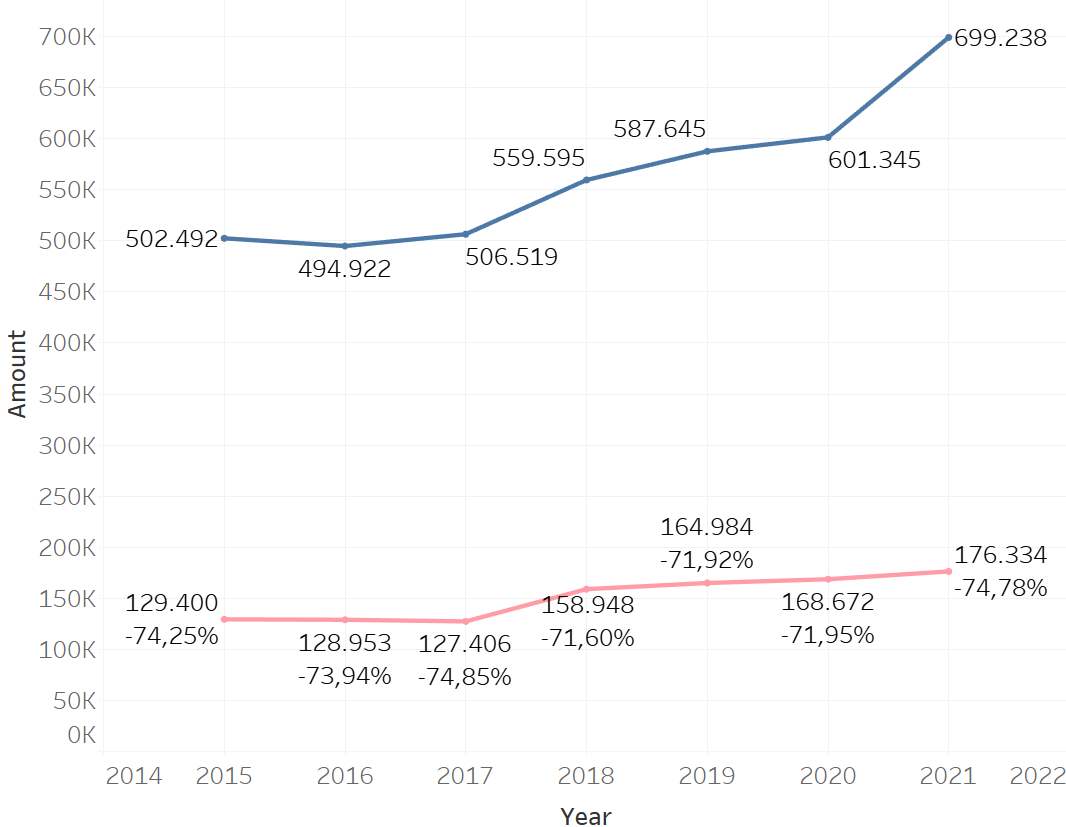
\includegraphics[width=85mm]{assets/1_qnt.PNG}
	}
	\caption{Quantidade geral}
	\label{fig_1_qnt}
\end{figure}

\subsubsection{Média salarial}

No gráfico da Figura \ref{fig_1_sal}, é possível verificar que em todos os anos a média salarial dos homens é maior que a das mulheres. Essa diferença era menor em 2015, cujo valor era de 4.87\%. Em 2021, essa diferença aumentou para 13.71\% e em 2021 ela voltou a diminuir e foi para 11.56\%.

\begin{figure}[htbp]
	\centerline{
		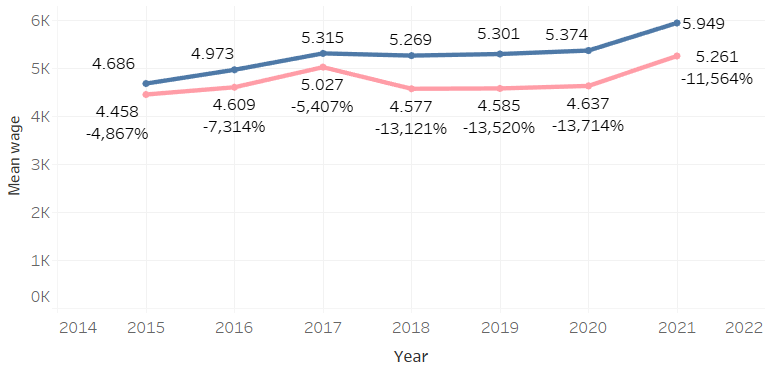
\includegraphics[width=85mm]{assets/1_sal.PNG}
	}
	\caption{Média salarial geral}
	\label{fig_1_sal}
\end{figure}


\subsection{Análise por nível educacional}  \label{sub:educ}

\subsubsection{Quantidade}

Na Figura \ref{fig_2_qnt_educ}, pode-se perceber que para os dois gêneros há um número maior de profissionais com ensino superior comparado ao número de profissionais apenas com ensino médio completo. A diferença entre os quantitativos de profissionais por gênero, tanto no nível médio como no superior, varia entre 71 e 78\%, sendo um pouco maior no nível médio.

\begin{figure}[htbp]
	\centerline{
		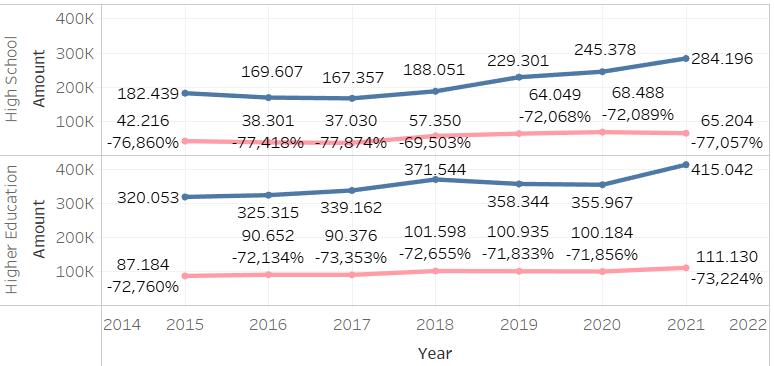
\includegraphics[width=85mm]{assets/2_qnt_educ.PNG}
	}
	\caption{Quantidade por nível educacional}
	\label{fig_2_qnt_educ}
\end{figure}

\subsubsection{Média salarial}

Para média salarial apresentada na Figura \ref{fig_2_sal_educ}, é possível verificar que em todos os anos a diferença salarial foi maior no nível médioquando comparado ao superior. Ou seja, a qualificação da mulher parece contribuir com a redução da desigualdade salarial entre os gêneros na TI.

\begin{figure}[htbp]
	\centerline{
		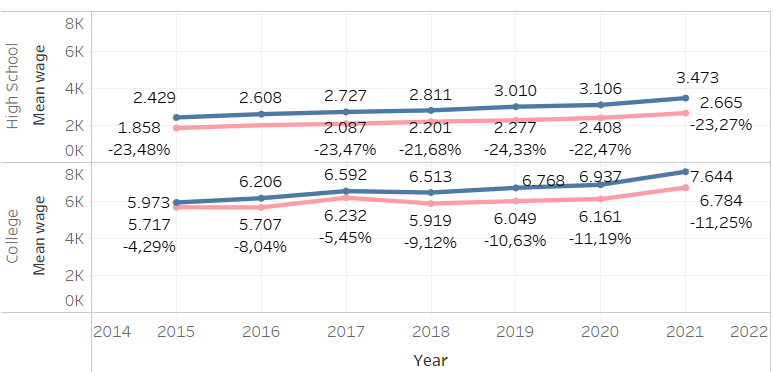
\includegraphics[width=85mm]{assets/2_sal_educ.PNG}
	}
	\caption{Média salarial por nível educacional}
	\label{fig_2_sal_educ}
\end{figure}

\subsection{Análise por setor privado e público}  \label{sub:privpub}

\subsubsection{Quantidade}

Nas Figuras \ref{fig_3_qnt_pubpriv} e \ref{fig_3_1_qnt_pubpriv} é possível verificar que a quantidade de profissionais do sexo masculino é superior à quantidade de profissionais do sexo feminino, independente do setor, público ou privado. Contudo, no setor privado a diferença é ainda maior, como no caso de 2021, onde essa diferença era de 75,19\%, enquanto que no setor público era de 61,09\%.

\begin{figure}[htbp]
	\centerline{
		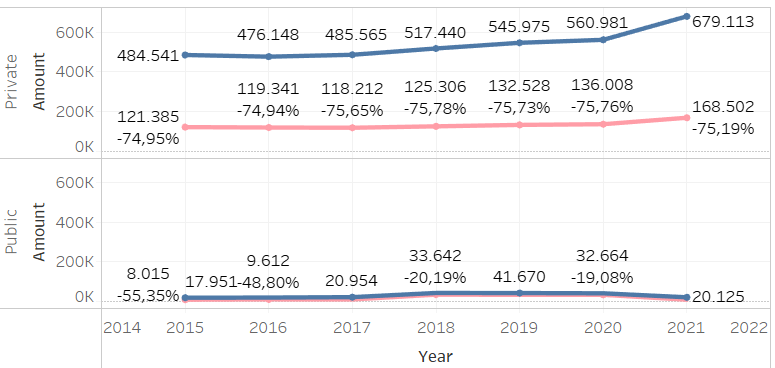
\includegraphics[width=85mm]{assets/3_qnt_pubpriv.PNG}
	}
	\caption{Quantidade por setor}
	\label{fig_3_qnt_pubpriv}
\end{figure}


\begin{figure}[htbp]
	\centerline{
		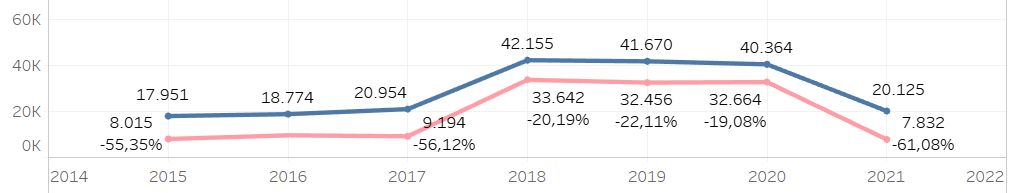
\includegraphics[width=85mm]{assets/3_1_qnt_pubpriv.PNG}
	}
	\caption{Gráfico ampliado da quantidade por setor público}
	\label{fig_3_1_qnt_pubpriv}
\end{figure}

\subsubsection{Média salarial}

Com relação às médias salariais apresentadas na Figura \ref{fig_3_sal_pubpriv}, as suas diferenças percentuais se apresentam similares quando se compara o setor privado com o quadro geral da Figura \ref{fig_1_sal}. Entretanto, ocorre uma discrepância muito maior nas diferenças percentuais entre os anos de 2018 e 2020 quando se olha para o setor público, mas os dados analisados não permitem identificar uma possível causa para esse fenômeno.

\begin{figure}[htbp]
	\centerline{
		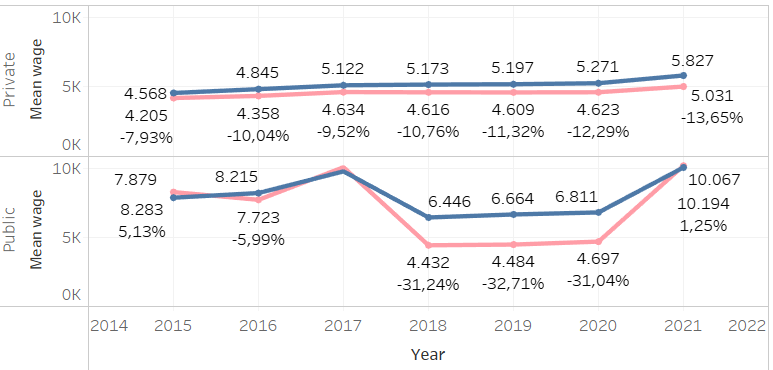
\includegraphics[width=85mm]{assets/3_sal_pubpriv.PNG}
	}
	\caption{Média salarial por setor}
	\label{fig_3_sal_pubpriv}
\end{figure}

\subsection{Quantidade de demissões}

Esta seção analisa de forma diferente das anteriormente expostas. Há um gráfico para cada gênero. Em cada gráfico, há a quantidade de pessoas demitidas e, logo abaixo, a de pessoas não demitidas, ou seja, mantidas no emprego no respectivo ano. A porcentagem é também diferente, pois analisa a diferença em relação ao dado anterior da própria linha, e não em relação ao outro sexo.

\subsubsection{Homem}

Destacamos aqui na Figura \ref{fig_4_qnt_h_demit} que o aumento de 35,82\% em 2021 foi o maior entre os outros anos. Isso mostra que a quantidade de demissões aumentou muito em relação ao ano anterior, que era de 116.604 demissões. 

\begin{figure}[htbp]
	\centerline{
		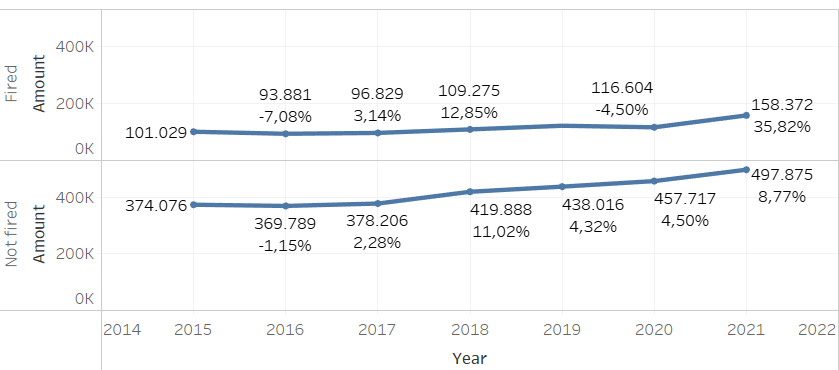
\includegraphics[width=85mm]{assets/4_qnt_h_demit.PNG}
	}
	\caption{Demissões de homens}
	\label{fig_4_qnt_h_demit}
\end{figure}

\subsubsection{Mulher}

Na Figura \ref{fig_4_qnt_m_demit}, é perceptível o mesmo aumento do gráfico anterior, porém com uma porcentagem de 29,91\% em relação a 2020. O grande número de demissões acontece em um ano em que a pandemia ainda estava em vigor. 

\begin{figure}[htbp]
	\centerline{
		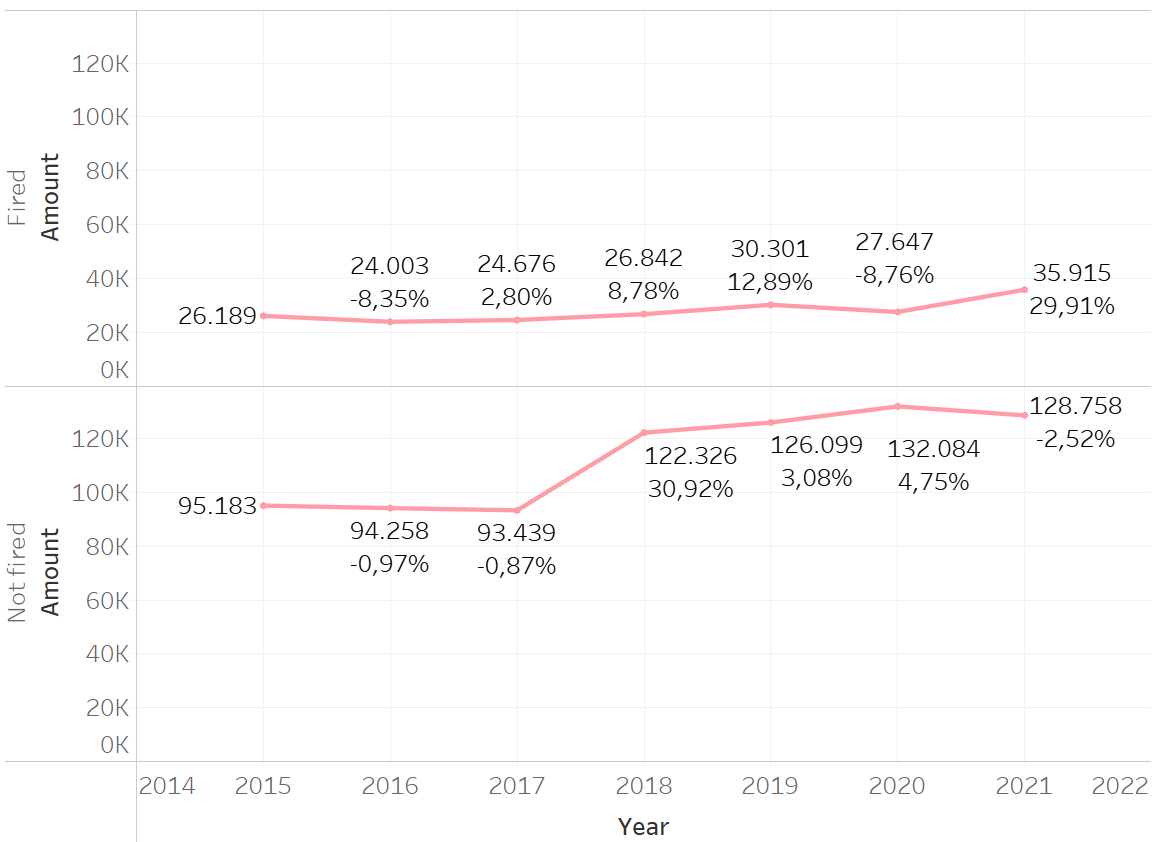
\includegraphics[width=85mm]{assets/4_qnt_m_demit.PNG}
	}
	\caption{Demissões de mulheres}
	\label{fig_4_qnt_m_demit}
\end{figure}

\subsection{Por cargo de TI}

Nas análises por cargos abaixo, consideramos apenas o ano de 2021, pois é o último ano disponível em nossa análise.

\subsubsection{Quantidade}

Podemos ver na Figura \ref{fig_5_qnt_cbo} abaixo que a quantidade de Analistas de Desenvolvimento de Sistemas é a que concentra a maior quantidade de profissionais, seguido por Analistas de Suporte Computacional, isso em ambos os sexos. 

\subsubsection{Média salarial}

Já na Figura \ref{fig_5_sal_cbo} é visível a diferença de salário entre o cargo com maior média e os demais. Portanto, para o cargo de Engenheiros de Sistemas Operacionais em Computação, há uma diferença de mais de 1.000 reais entre os sexos. Porém há um dado curioso, no cargo de Analista de Redes e de Comunicação de Dados há um ligeiro ganho salarial para as mulheres. Enquanto que para os homens é de 6.233 reais, para as mulheres é de 6.270 reais, ou seja, uma diferença de 2,17\% a mais para as mulheres.

\begin{figure}[htbp]
	\centerline{
		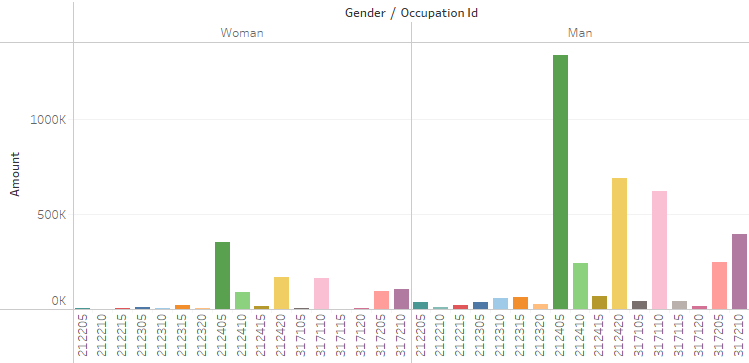
\includegraphics[width=85mm]{assets/5_qnt_cbo.PNG}
	}
	\caption{Quantidade por cargo em 2021}
	\label{fig_5_qnt_cbo}
\end{figure}

\begin{figure}[htbp]
	\centerline{
		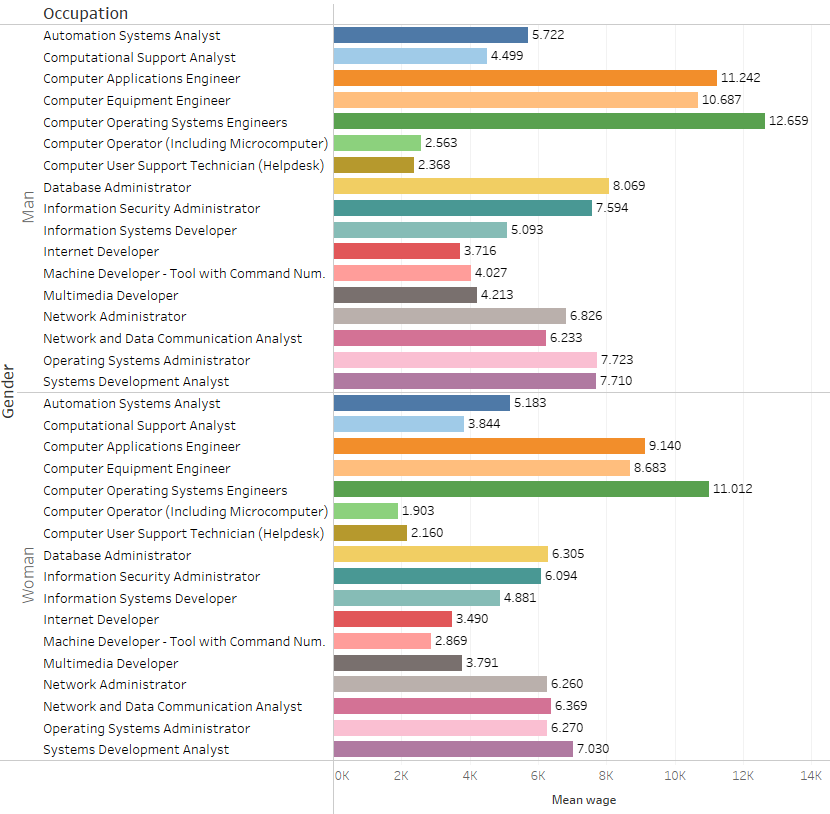
\includegraphics[width=85mm]{assets/5_sal_cbo.PNG}
	}
	\caption{Média salarial por cargo em 2021}
	\label{fig_5_sal_cbo}
\end{figure}